% Options for packages loaded elsewhere
% Options for packages loaded elsewhere
\PassOptionsToPackage{unicode}{hyperref}
\PassOptionsToPackage{hyphens}{url}
\PassOptionsToPackage{dvipsnames,svgnames,x11names}{xcolor}
%
\documentclass[
  letterpaper,
  DIV=11,
  numbers=noendperiod]{scrreprt}
\usepackage{xcolor}
\usepackage{amsmath,amssymb}
\setcounter{secnumdepth}{5}
\usepackage{iftex}
\ifPDFTeX
  \usepackage[T1]{fontenc}
  \usepackage[utf8]{inputenc}
  \usepackage{textcomp} % provide euro and other symbols
\else % if luatex or xetex
  \usepackage{unicode-math} % this also loads fontspec
  \defaultfontfeatures{Scale=MatchLowercase}
  \defaultfontfeatures[\rmfamily]{Ligatures=TeX,Scale=1}
\fi
\usepackage{lmodern}
\ifPDFTeX\else
  % xetex/luatex font selection
\fi
% Use upquote if available, for straight quotes in verbatim environments
\IfFileExists{upquote.sty}{\usepackage{upquote}}{}
\IfFileExists{microtype.sty}{% use microtype if available
  \usepackage[]{microtype}
  \UseMicrotypeSet[protrusion]{basicmath} % disable protrusion for tt fonts
}{}
\makeatletter
\@ifundefined{KOMAClassName}{% if non-KOMA class
  \IfFileExists{parskip.sty}{%
    \usepackage{parskip}
  }{% else
    \setlength{\parindent}{0pt}
    \setlength{\parskip}{6pt plus 2pt minus 1pt}}
}{% if KOMA class
  \KOMAoptions{parskip=half}}
\makeatother
% Make \paragraph and \subparagraph free-standing
\makeatletter
\ifx\paragraph\undefined\else
  \let\oldparagraph\paragraph
  \renewcommand{\paragraph}{
    \@ifstar
      \xxxParagraphStar
      \xxxParagraphNoStar
  }
  \newcommand{\xxxParagraphStar}[1]{\oldparagraph*{#1}\mbox{}}
  \newcommand{\xxxParagraphNoStar}[1]{\oldparagraph{#1}\mbox{}}
\fi
\ifx\subparagraph\undefined\else
  \let\oldsubparagraph\subparagraph
  \renewcommand{\subparagraph}{
    \@ifstar
      \xxxSubParagraphStar
      \xxxSubParagraphNoStar
  }
  \newcommand{\xxxSubParagraphStar}[1]{\oldsubparagraph*{#1}\mbox{}}
  \newcommand{\xxxSubParagraphNoStar}[1]{\oldsubparagraph{#1}\mbox{}}
\fi
\makeatother


\usepackage{longtable,booktabs,array}
\usepackage{calc} % for calculating minipage widths
% Correct order of tables after \paragraph or \subparagraph
\usepackage{etoolbox}
\makeatletter
\patchcmd\longtable{\par}{\if@noskipsec\mbox{}\fi\par}{}{}
\makeatother
% Allow footnotes in longtable head/foot
\IfFileExists{footnotehyper.sty}{\usepackage{footnotehyper}}{\usepackage{footnote}}
\makesavenoteenv{longtable}
\usepackage{graphicx}
\makeatletter
\newsavebox\pandoc@box
\newcommand*\pandocbounded[1]{% scales image to fit in text height/width
  \sbox\pandoc@box{#1}%
  \Gscale@div\@tempa{\textheight}{\dimexpr\ht\pandoc@box+\dp\pandoc@box\relax}%
  \Gscale@div\@tempb{\linewidth}{\wd\pandoc@box}%
  \ifdim\@tempb\p@<\@tempa\p@\let\@tempa\@tempb\fi% select the smaller of both
  \ifdim\@tempa\p@<\p@\scalebox{\@tempa}{\usebox\pandoc@box}%
  \else\usebox{\pandoc@box}%
  \fi%
}
% Set default figure placement to htbp
\def\fps@figure{htbp}
\makeatother





\setlength{\emergencystretch}{3em} % prevent overfull lines

\providecommand{\tightlist}{%
  \setlength{\itemsep}{0pt}\setlength{\parskip}{0pt}}



 


\KOMAoption{captions}{tableheading}
\makeatletter
\@ifpackageloaded{bookmark}{}{\usepackage{bookmark}}
\makeatother
\makeatletter
\@ifpackageloaded{caption}{}{\usepackage{caption}}
\AtBeginDocument{%
\ifdefined\contentsname
  \renewcommand*\contentsname{Table of contents}
\else
  \newcommand\contentsname{Table of contents}
\fi
\ifdefined\listfigurename
  \renewcommand*\listfigurename{List of Figures}
\else
  \newcommand\listfigurename{List of Figures}
\fi
\ifdefined\listtablename
  \renewcommand*\listtablename{List of Tables}
\else
  \newcommand\listtablename{List of Tables}
\fi
\ifdefined\figurename
  \renewcommand*\figurename{Figure}
\else
  \newcommand\figurename{Figure}
\fi
\ifdefined\tablename
  \renewcommand*\tablename{Table}
\else
  \newcommand\tablename{Table}
\fi
}
\@ifpackageloaded{float}{}{\usepackage{float}}
\floatstyle{ruled}
\@ifundefined{c@chapter}{\newfloat{codelisting}{h}{lop}}{\newfloat{codelisting}{h}{lop}[chapter]}
\floatname{codelisting}{Listing}
\newcommand*\listoflistings{\listof{codelisting}{List of Listings}}
\makeatother
\makeatletter
\makeatother
\makeatletter
\@ifpackageloaded{caption}{}{\usepackage{caption}}
\@ifpackageloaded{subcaption}{}{\usepackage{subcaption}}
\makeatother
\usepackage{bookmark}
\IfFileExists{xurl.sty}{\usepackage{xurl}}{} % add URL line breaks if available
\urlstyle{same}
\hypersetup{
  pdftitle={Alfaza Naufal Zakiy},
  pdfauthor={18222126 Alfaza Naufal Zakiy},
  colorlinks=true,
  linkcolor={blue},
  filecolor={Maroon},
  citecolor={Blue},
  urlcolor={Blue},
  pdfcreator={LaTeX via pandoc}}


\title{Alfaza Naufal Zakiy}
\usepackage{etoolbox}
\makeatletter
\providecommand{\subtitle}[1]{% add subtitle to \maketitle
  \apptocmd{\@title}{\par {\large #1 \par}}{}{}
}
\makeatother
\subtitle{Portfolio Asesmen II-2100 KIPP}
\author{18222126 Alfaza Naufal Zakiy}
\date{2025-09-15}
\begin{document}
\maketitle

\renewcommand*\contentsname{Table of contents}
{
\hypersetup{linkcolor=}
\setcounter{tocdepth}{2}
\tableofcontents
}

\bookmarksetup{startatroot}

\chapter*{Selamat Datang}\label{selamat-datang}
\addcontentsline{toc}{chapter}{Selamat Datang}

\markboth{Selamat Datang}{Selamat Datang}

Saya Alfaza Naufal Zakiy (18222126), mahasiswa Program Studi Sistem dan
Teknologi Informasi, Sekolah Teknik Elektro dan Informatika -- Institut
Teknologi Bandung (ITB).

Website ini dibuat sebagai bagian dari asesmen mata kuliah II2100
Komunikasi Interpersonal dan Publik (KIPP) yang berfokus pada
pengembangan kemampuan berkomunikasi secara efektif, reflektif, dan
bermakna dalam konteks akademik maupun profesional.

Melalui laman ini, saya membagikan proses belajar, refleksi diri, serta
karya-karya yang menggambarkan perjalanan saya dalam memahami esensi
komunikasi interpersonal---mulai dari kesadaran diri, empati, hingga
kemampuan menyampaikan gagasan secara terbuka dan konstruktif.

Setiap bagian di website ini dirancang untuk menunjukkan bahwa
komunikasi bukan sekadar keterampilan berbicara, tetapi juga seni
membangun hubungan dan menciptakan pemahaman bersama melalui setiap kata
dan tindakan.

\bookmarksetup{startatroot}

\chapter{UTS-1 All About Me}\label{uts-1-all-about-me}

\begin{figure}[H]

{\centering 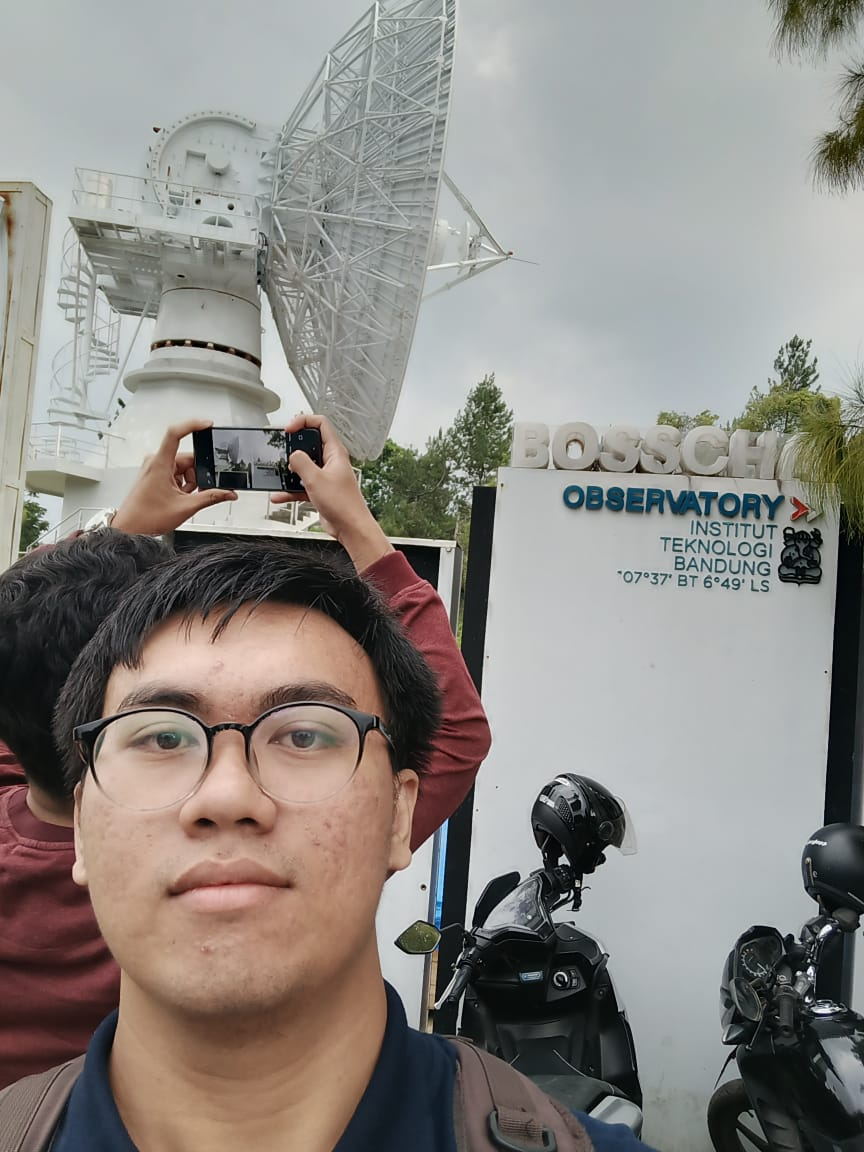
\includegraphics[width=0.5\linewidth,height=\textheight,keepaspectratio]{All_About_me/../images/zakiy.jpeg}

}

\caption{About Me}

\end{figure}%

Halo semuannya salam kenal 😊, Perkenalkan Nama saya Alfaza Naufal
Zakiy, teman-teman biasanya memanggil saya Zakiy, Zek, atau kadang Jack.
Saya mahasiswa Sistem dan Teknologi Informasi di ITB. Saya tipe orang
yang selalu ingin tahu bagaimana sesuatu bekerja. Sering kali saya lebih
sibuk berpikir dan mengamati daripada ikut obrolan yang tidak jelas
arahnya. Saya merasa itu yang membuat saya berbeda, karena saya suka
mencari makna di balik hal-hal kecil.

Sekarang fokus utama saya adalah belajar. Tidak hanya belajar akademik
di kampus, tapi juga belajar memahami diri saya sendiri. Saya lebih suka
membandingkan diri saya hari ini dengan diri saya kemarin daripada
membandingkan diri dengan orang lain. Dari situ saya bisa melihat
kemajuan kecil yang mungkin tidak terlihat oleh orang lain, tapi berarti
banyak buat saya.

Dalam berkomunikasi, saya cukup empatik, suka mendengarkan, dan terbiasa
menyampaikan sesuatu dengan padat dan jelas. Saat ini saya sedang
berlatih untuk berbicara lebih percaya diri, membaca bahasa tubuh orang
lain, dan memahami makna yang tidak selalu diucapkan secara langsung. Di
luar itu, saya juga sedang belajar mengatur waktu dengan lebih baik,
karena sering kali saya menyesal setelah menyadari waktu saya terbuang
untuk hal yang kurang penting. Nilai komunikasi yang paling saya pegang
adalah empati, kejujuran, dan kejelasan.

\section{Momen dan Pelajaran}\label{momen-dan-pelajaran}

Saya pernah ada di situasi di mana saya takut bertemu teman sekelas
sendiri karena sempat melakukan kesalahan. Waktu itu saya memilih untuk
menghindar. Hasilnya, memang terasa lega sesaat, tapi saya juga
kehilangan kesempatan untuk memperbaiki hubungan. Dari situ saya belajar
bahwa menghindar tidak pernah menyelesaikan apa pun. Kalau salah, lebih
baik diakui dan dihadapi. Rasa malu biasanya hanya di awal, tapi rasa
lega datang setelahnya.

Ada juga momen ketika ekspektasi saya terhadap teman tidak sesuai dengan
kenyataan. Saya mencoba mengalihkan pikiran dengan bekerja di depan
laptop, tapi perasaan sedih tetap datang. Akhirnya saya menangis selama
lima menit, bukan karena lemah, tapi karena terlalu lelah menahan
semuanya sendiri. Dari situ saya belajar bahwa konflik yang dibiarkan
berlarut-larut hanya membuat capek. Kadang yang kita butuh bukan
pembenaran, tapi penerimaan bahwa keadaan memang tidak selalu sesuai
harapan.

Pernah juga saya menghadapi situasi saat harus mengerjakan UTS take home
dan waktu hampir habis. Saya panik, bekerja dengan terburu-buru, dan
akhirnya banyak fitur yang tidak berjalan. Dari situ saya belajar
pentingnya memprioritaskan tugas. Sekarang saya terbiasa memilah
pekerjaan dengan bantuan prinsip Urgent-Important Matrix agar bisa fokus
pada hal yang benar-benar penting.

Setelah ikut mata kuliah KIPP, cara pandang saya terhadap komunikasi
berubah cukup banyak. Saya mulai sadar bahwa sikap, ekspresi, dan bahasa
tubuh punya pengaruh besar. Sekarang saya lebih berusaha memahami makna
dari apa yang orang lain sampaikan, melihatnya dari berbagai sudut
pandang, bukan hanya dari sudut pandang saya sendiri.

\section{Presentasi dan Cara Bicara}\label{presentasi-dan-cara-bicara}

Dulu saya takut sekali presentasi. Saya tipe orang yang perlu waktu
berpikir panjang sebelum bicara, jadi kalau ada pertanyaan sulit, saya
sering diam cukup lama. Saat itu saya suka membaca slide karena isinya
terlalu penuh. Sekarang saya belajar tampil lebih ringan. Saya hanya
menuliskan poin penting dan benar-benar memahami materi sebelum
presentasi, supaya penjelasannya tetap mengalir.

Pesan utama favorit saya saat presentasi adalah ``Jalanin aja dulu.''
Buat saya, kalimat ini sederhana tapi bermakna dalam. Tidak perlu
menunggu sempurna untuk mulai, yang penting berani mencoba. Kesempurnaan
akan datang lewat prosesnya. Pesan ini saya gunakan juga untuk
mengingatkan diri sendiri agar tidak menunda.

Untuk melakukan pembukaan presentasi yang menarik dan fresh, saya suka
memakai kalimat kontras yang sederhana. Pernah saya membuka presentasi
dengan kalimat ``Banyak orang takut gagal, tapi saya percaya mending
menyesal mencoba daripada menyesal tidak mencoba.'' Biasanya audiens
langsung senyum dan fokus mendengarkan.

Saya bukan orang yang suka melucu di depan umum, jadi cara saya
mencairkan suasana biasanya lewat senyum, nada bicara yang hangat, dan
kontak mata. Kadang saya menambahkan cerita singkat yang relevan supaya
audiens tetap merasa dekat tanpa harus tertawa.

\section{Prinsip dan Refleksi}\label{prinsip-dan-refleksi}

Ada tiga prinsip utama yang selalu saya pegang, baik di kelas maupun di
luar kelas. Pertama, dengarkan dulu sebelum berbicara. Kedua, jelaskan
niat sebelum memberi saran. Ketiga, sampaikan hal sulit dengan tenang
dan jelas.

Menurut saya, komunikasi itu seperti jaringan data. Kalau sinyalnya
buruk, pesan bisa salah diterima. Maka saya berusaha memastikan
``jaringan'' antara saya dan orang lain tetap stabil dengan cara
mendengarkan baik-baik, mengklarifikasi, dan memastikan pesannya
tersampaikan dengan jelas.

Saya juga berusaha menyeimbangkan antara fakta dan empati. Misalnya,
ketika teman saya melakukan kesalahan, saya tidak langsung bilang ``kamu
salah'', tapi saya mulai dengan kalimat ``Aku ngerti maksudmu, tapi
mungkin di bagian ini bisa kita cek lagi datanya.'' Dengan begitu, pesan
bisa sampai tanpa membuat orang merasa diserang.

Kalimat yang paling bermakna buat saya adalah ``Remember why you
started.'' Setiap kali saya merasa lelah atau ingin menyerah, kalimat
itu selalu mengingatkan saya untuk kembali pada alasan awal saya
memulai. Bukan untuk menjadi sempurna, tapi untuk menjadi lebih baik
dari kemarin.

\section{Penutup}\label{penutup}

Akhirnya kita masuk di bagian paling akhir di bagian UTS-1 All About Me.
Kalau saya boleh menyimpulkan perjalanan saya di mata kuliah KIPP,
mungkin satu kata yang paling pas adalah ``berproses.'' Saya belajar
bahwa komunikasi bukan cuma soal berbicara, tapi juga tentang bagaimana
kita hadir sepenuhnya di hadapan orang lain. Kadang cukup dengan
mendengarkan, tersenyum, atau jujur mengungkapkan perasaan kita.

Melalui tugas ini, saya ingin berbagi perjalanan kecil saya sebagai
seseorang yang dulunya sering overthinking sebelum bicara, dan kini
sedang belajar untuk lebih terbuka serta berani menyampaikan pikiran
dengan tulus.

Terima kasih sudah membaca cerita ini. Kalau ada masukan, saya akan
sangat senang mendengarnya. Karena bagi saya, komunikasi yang baik tidak
berhenti di kata-kata yang diucapkan, tapi terus hidup dari apa yang
kita dengar setelahnya.

\bookmarksetup{startatroot}

\chapter{UTS-2 My Songs for You}\label{uts-2-my-songs-for-you}

Untuk temanku tercinta Lirik by Alfaza Naufal Zakiy

Music: SUNO

File Lagu
\url{https://drive.google.com/file/d/1CEcoW-aY6Kv-ebu0mIWvEDLoR2dyvzwx/preview}

Lirik

{[}Verse 1{]}

Waktu berjalan pelan, ku duduk mengenang

Tentang hari saat kau bilang ``nggak apa-apa, ayo jalan''

Kau yang jarang bicara, tapi matamu tenang

Mengingatkanku, kuat tak harus lantang

{[}Pre-Chorus{]}

Saat dunia berisik dan aku nyaris hilang arah

Kau tetap di sana, tanpa banyak kata

{[}Chorus{]}

Terima kasih sudah tinggal

Saat dunia terasa kejam dan asing

Kau tunjukkan arti sederhana

Bahwa hadir itu lebih dari sekadar datang

Kau buktikan cinta tak harus diucapkan

Cukup ada, dan aku paham

{[}Verse 2{]}

Pernah ku jatuh, hampir menyerah

Tapi suaramu hadir, ringan tapi nyata

Kau bilang ``nggak semua luka harus disembunyikan''

Dan malam itu jadi awal aku belajar bertahan

{[}Pre-Chorus{]}

Kau bukan penyelamat, tapi pengingat kecil

Bahwa manusia cukup dengan saling menguatkan

{[}Chorus{]}

Terima kasih sudah tinggal

Saat dunia terasa kejam dan asing

Kau tunjukkan arti sederhana

Bahwa hadir itu lebih dari sekadar datang

Kau buktikan cinta tak harus diucapkan

Cukup ada, dan aku paham

{[}Bridge{]}

Kalau nanti aku lupa cara bersyukur

Ingatkan aku dengan senyummu yang jujur

Dan kalau aku tersesat lagi

Biarlah lagu ini jadi peta untuk kembal

{[}Final Chorus{]}

Terima kasih sudah tinggal

Bahkan saat semua terasa berat

Kau tunjukkan bahwa cahaya

Bisa lahir dari orang yang diam-diam kuat

Kau ajarkan arti sabar dan tulus

Dan aku ingin kamu tahu

Lagu ini, ditulis untukmu

{[}Outro{]}

Tak semua pahlawan bersuara lantang

Kadang cukup satu senyum yang tenang

Terima kasih, untuk diam yang menguatkan

``My Songs for You'' adalah caraku membalas dengan perasaan

\bookmarksetup{startatroot}

\chapter{UTS-3 My Stories for You}\label{uts-3-my-stories-for-you}

\section{Cerita Inspiratif}\label{cerita-inspiratif}

Tahun 2022 menjadi titik baru dalam hidup saya. Hari itu saya menerima
kabar bahwa saya diterima di ITB. Kabar yang begitu membahagiakan, bukan
hanya bagi saya, tapi juga orang-orang di sekitar saya. Tidak pernah
saya bayangkan bisa menapaki kampus yang selama ini hanya saya dengar
dari cerita orang. Saya datang ke Bandung dengan hati berbunga-bunga,
penuh semangat untuk memulai kehidupan baru.

Namun, kenyataannya tidak seindah yang saya pikirkan. Perubahan
lingkungan, ritme hidup yang berbeda, dan suasana akademik yang begitu
menantang membuat saya mengalami culture shock. Saya yang terbiasa hidup
dalam rutinitas terarah tiba-tiba kehilangan pegangan. Hari-hari yang
awalnya penuh antusiasme perlahan berubah menjadi rasa cemas, minder,
dan bahkan depresi. Saya merasa tertinggal jauh dari teman-teman yang
tampak cepat beradaptasi. Rasa percaya diri saya runtuh. Dalam diam,
saya merasa seperti orang paling bodoh di antara mereka. Sampai di titik
di mana saya mulai berpikir saya tidak lagi berharga.

Saya mengurung diri dan mulai menjauh dari teman-teman. Tidak ada lagi
yang mencoba menyapa atau menanyakan kabar saya, setidaknya begitu yang
saya rasakan. Di momen itu, dunia terasa sunyi sekali. Tapi, di balik
kesunyian itu, semesta seperti ingin menegur saya dengan cara yang
lembut.

\section{Titik Balik}\label{titik-balik}

Beberapa waktu kemudian, saya mulai mendapatkan sedikit cahaya dari
orang-orang yang masih peduli. Teman-teman saya di Malang masih sering
mengirim pesan dan menanyakan kabar, meski saya jarang membalas. Lalu
datang satu momen yang tidak akan pernah saya lupakan: sebuah nasihat
dari ayah teman kakak saya.

Beliau berkata dengan nada tenang, ``Nggak apa-apa nilaimu nggak
bagus-bagus amat. Kamu udah masuk kampus ini aja udah hebat banget,
Zakiy.'' Kalimat itu menampar tapi juga menenangkan. Ia melanjutkan,
``Lebih baik terlihat bodoh di lingkungan orang pintar, daripada
terlihat pintar di lingkungan orang bodoh.'' Awalnya saya sempat
tersinggung, tapi setelah saya renungkan, saya sadar kalimat itu penuh
makna.

Tidak berhenti di situ, seseorang juga berkata pada saya, ``Jalanin aja
perkuliahanmu, jangan bandingin dirimu sama orang lain. Bandingin aja
dirimu hari ini sama dirimu kemarin. Sedikit kemajuan tetap kemajuan,
kan?'' Ucapan itu menjadi pelita kecil yang membuat saya mulai menatap
hari-hari berikutnya dengan lebih ringan.

\section{Perubahan}\label{perubahan}

Sejak saat itu, saya berusaha menikmati kehidupan dengan cara yang lebih
sederhana. Saya belajar untuk hidup di saat ini, bukan di masa lalu atau
di masa depan. Saya teringat kutipan dari Master Oogway di film Kung Fu
Panda: ``Yesterday is history, tomorrow is a mystery, and today is a
gift\ldots{} that's why they call it the present.''

Saya mulai belajar dengan kecepatan saya sendiri. Tidak perlu bersaing
dengan siapa pun, cukup berprogres sesuai kemampuan. Saya menargetkan
hal-hal yang realistis dan memberi ruang bagi diri saya untuk berkembang
pelan-pelan. Saya mulai lebih bersyukur, bahkan untuk hal-hal kecil:
penjual nasi di warteg yang selalu menyapa, tukang laundry yang ramah,
tumbuhan di depan kos, sampai kucing yang sering datang tanpa permisi.

Saya sadar bahwa kita semua bermanfaat bagi lingkungan sekitar, hanya
saja kadang kita tidak menyadarinya. Saya juga mulai melatih diri
berbicara dengan orang lain tanpa takut salah, berani bertanya ke dosen,
dan tidak lagi khawatir jika orang lain menilai saya. Saya belajar bahwa
saya tidak bisa mengontrol reaksi orang lain, tapi saya bisa mengontrol
bagaimana saya merespons.

\section{Hasil dan Pembelajaran}\label{hasil-dan-pembelajaran}

Perlahan, rasa percaya diri saya mulai tumbuh kembali. Saya mulai
menikmati interaksi dengan orang lain, tidak lagi merasa kecil di tengah
orang-orang hebat. Energi saya tidak lagi habis untuk hal yang tidak
penting. Saya bisa fokus belajar, memahami materi, dan bersyukur ketika
melihat nilai-nilai saya yang terus meningkat dari waktu ke waktu. Itu
menjadi bukti kecil bahwa saya sudah berada di jalur yang tepat.

\section{Pesan untuk Pembaca}\label{pesan-untuk-pembaca}

Kalau boleh saya simpulkan, pelajaran terbesar dari perjalanan ini
adalah untuk selalu bangga pada diri sendiri. Jangan terlalu sering
membandingkan diri dengan orang lain, karena kita tidak pernah tahu
bagaimana perjuangan di balik layar kehidupan mereka. Banyak orang hanya
menampilkan kesuksesannya di media sosial, sementara kegagalannya
disembunyikan. Tanpa sadar, kita membandingkan seluruh perjalanan hidup
kita dengan ``cuplikan terbaik'' orang lain.

Banggalah pada setiap langkah kecil yang kamu ambil, sekecil apa pun
itu. Karena tidak semua kemajuan terlihat besar, dan tidak semua
keberhasilan perlu diumumkan.

\section{Nilai dan Makna}\label{nilai-dan-makna}

Cerita ini mengajarkan saya tentang empati pada diri sendiri. Saya
belajar untuk menerima bahwa tidak apa-apa tidak selalu baik-baik saja.
Fokuslah pada diri sendiri, lakukan tindakan nyata, dan percayalah pada
proses yang sedang berjalan. Kita tidak perlu memaksakan kecepatan kita
agar sama dengan orang lain. Yang terpenting, kita terus melangkah dan
tidak berhenti.

\section{Nuansa Emosi}\label{nuansa-emosi}

Ketika menulis ini, saya masih bisa mengingat jelas campuran perasaan
yang dulu saya rasakan: takut, malu, lalu perlahan berganti menjadi
lega, terharu, bangga, dan akhirnya bahagia.

\section{Penutup}\label{penutup-1}

Semoga cerita ini bisa mengingatkan siapa pun yang membaca untuk tetap
percaya pada diri sendiri dan menghargai setiap proses, sekecil apa pun
itu. Jangan menunggu orang lain yang datang untuk menyemangati kamu,
karena kekuatan terbesar justru muncul saat kamu mulai menguatkan diri
sendiri.

\emph{Be proud of yourself --- kamu berharga, bahkan ketika kamu belum
menyadarinya.}

\bookmarksetup{startatroot}

\chapter{UTS-4 My SHAPE (Spiritual Gifts, Heart, Abilities, Personality,
Experiences)}\label{uts-4-my-shape-spiritual-gifts-heart-abilities-personality-experiences}

TBD

\bookmarksetup{startatroot}

\chapter{UTS-5 My Personal Reviews}\label{uts-5-my-personal-reviews}

TBD

\bookmarksetup{startatroot}

\chapter{UAS-1 My Concepts}\label{uas-1-my-concepts}

TBD

\bookmarksetup{startatroot}

\chapter{UAS-3 My Opinions}\label{uas-3-my-opinions}

TBD

\bookmarksetup{startatroot}

\chapter{UAS-3 My Innovations}\label{uas-3-my-innovations}

TBD

\bookmarksetup{startatroot}

\chapter{UAS-4 My Knowledge}\label{uas-4-my-knowledge}

TBD

\bookmarksetup{startatroot}

\chapter{UAS-5 My Professional
Reviews}\label{uas-5-my-professional-reviews}

TBD

\bookmarksetup{startatroot}

\chapter{Summary}\label{summary}

TBD

\bookmarksetup{startatroot}

\chapter*{References}\label{references}
\addcontentsline{toc}{chapter}{References}

\markboth{References}{References}

\phantomsection\label{refs}




\end{document}
